Le choix de l'architecture a été guidé par les considérations suivantes:
\begin{itemize}
    \item   Il y aura qu'un seul utilisateur: aucun niveau d'accès à gérer.
    \item   Le système ne devra pas être réparti sur plusieurs machines.
    \item   le système n'offrira pas de services réseau à des clients.
    \item   Le problème peut être décomposé en sous-problèmes indépendants les uns des autres.
\end{itemize}

Une architecture modulaire a été conçue pour implémenter le prototype de manière à préserver l'indépendance des différentes sections. Ce choix a été fait pour des raisons techniques et contextuelles.

D'un point de vue technique, la conception modulaire a été faite de manière à limiter le couplage entre les modules et augmenter la cohésion des différents modules. Ces propriétés sont recherchées puisqu'elles supposent une application plus facile à maintenir et faire évoluer. Pour atteindre ces propriétés, les modules seront conçus de manière à exposer une interface cohérente et la communication entre les modules sera faite par cette interface.

Tim O'Reilly a écrit en 2004 que les projets \emph{open source} qui connaissent le plus de succès sont ceux qui sont faits selon une architecture de participation~\cite{oreillyarchitecture}. Pour qu'il y ait architecture participative, les modules doivent être suffisamment cohérents et indépendants pour qu'un tiers puisse en extraire et en utiliser un, dans une autre solution, sans avoir besoin d'utiliser les autres modules.

Par exemple, une personne tierce pourrait avoir un ensemble de besoins différents de l'ensemble de besoins auxquels le prototype répond. Elle pourrait être par contre intéressée par le module d'acquisition de références bibliographiques. Une architecture de participation en est une qui permettrait aisément à cette personne d'utiliser ce module pour répondre à ses propres besoins, l'améliorer si elle en a besoin et ensuite contribuer à l'amélioration du composant en fournissant le code source des modifications. L'idée fondamentale derrière cette architecture est qu'il est plus simple pour la personne tierce d'utiliser un module existant plutôt que d'en développer un nouveau, et que le créateur initial tire aussi un bénéfice de cette collaboration. 

\subsubsection{Diagramme de paquetage}
Une vue de haut niveau du découpage en paquetages est présentée à la figure~\ref{paquetages} Voici une brève description des différents paquets.

\subsubsection{Diagramme des modules}
\begin{figure}
    \centerline{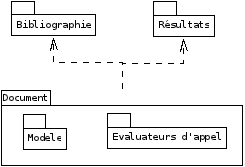
\includegraphics{figures/diagramme-paquetage.png}}
    \caption{Découpage en paquetages du prototype}
    \label{paquetages}
\end{figure}
\begin{itemize}
    \item Document - contient le modèle et les évaluateurs d'appel;
    \item Bibliographie - contient ce qui a trait à l'extraction des métadonnées des citations et l'acquisition de ressources en ligne;
    \item Résultats - classes pour analyser les résultats des évaluateurs d'appels. 
\end{itemize}

\subsubsection{Diagramme de classe du modèle}
Le diagramme de classe du modèle est présenté à la page~\ref{classesmodele}. En python, les méthodes de classe prennent comme premier paramètre l'instance sur laquelle elles s'appliquent. Ce paramètre est le premier paramètre qui est passé à la méthode et est généralement nommé \emph{self}. Il a été omis du diagramme pour améliorer la lisibilité.

Les classes du modèle sont liées par une relation de composition allant du général au particulier. Les classes les plus générales encapsulent les classes les plus particulières et calculent des statistiques à leur égard.

\begin{figure}
    \centerline{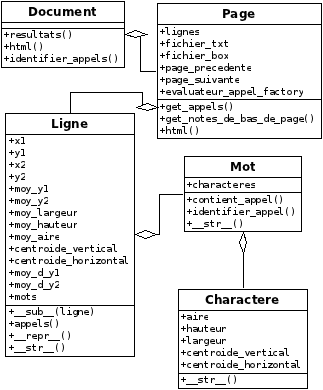
\includegraphics{figures/diagramme-classe-modele.png}}
    \caption{Diagramme de classes du modele}
    \label{classesmodele}
\end{figure}

\subsubsection{Diagramme de classe du module résultats}
Le module résultats contient deux classes: FichierRésultats et ComparateurResultats. FichierRésultats encapsule un \emph{parser} XML qui lit un fichier de résultats d'identification d'appels. \footnote{Le format de ce fichier est présenté dans la section \emph{Identification des appels}}. La méthode eq est implémentée pour surcharger l'opérateur "=": fichier1 = fichier2 retournera vrai si les deux ont identifié les mêmes appels dans les mêmes pages

La méthode compare initialise un ComparateurResultats à partir du résultat entre les deux fichiers. Le FichierRésultats sur lequel la méthode est appelée sera considéré comme la référence. Le diagramme de classes est présenté à la page~\ref{classesresultat}

\subsubsection{Diagramme de classe du module Evaluateurs d'appels}
L'implémentation du module d'évaluation d'appels repose sur le patron \emph{composite} et le patron \emph{factory} tels qu'identifiés par Gamma et \emph{al.} dans \emph{Design patterns}\cite{gamma1995design}. Une interface nommée \emph{EvaluateurAppel} spécifie que les évaluateurs d'appels devront implémenter une méthode \emph{isappel} prenant comme paramètre un caractère et dire si ce caractère est un appel de note de bas de page ou non; une série d'évaluateurs concrets encapsulant chacun une règle précise ont été implémentés. La classe \emph{EvaluateurComposite} est un évaluateur spécial qui contient plusieurs évaluateurs spécifiques et qui retourne "Vrai" si et seulement si tous ses évaluateurs retournent Vrai, ce qui permet de représenter des règles d'identifications complexes. En outre, il est possible de représenter diverses granularités de règles étant donné qu'un \emph{EvaluateurComposite} peut être encapsulé par un \emph{EvaluateurComposite} à son tour. La seule classe à être couplée à tous les évaluateurs concrets est la classe EvaluateurAppelFactory: celle-ci connaît les règles qui régissent l'identification des appels et peut créer un EvaluateurAppelComposite pour une page précise.

La logique spécifique des évaluateurs d'appels est décrite à la page~\pageref{tableau-evaluateurs}. Le diagramme de classe est présenté à la page~\pageref{classesresultat}
\begin{figure}
    \centerline{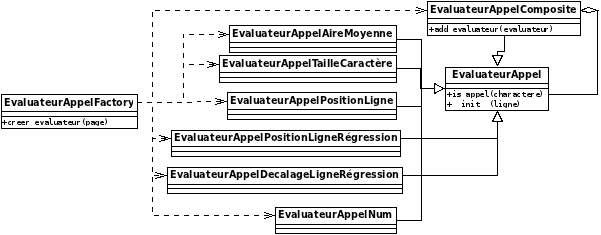
\includegraphics{figures/diagramme-classe-evaluateurs.png}}
    \caption{Diagramme de classes du module «Évaluateurs d'appels»}
    \label{classesevaluateurs}
\end{figure}


\begin{figure}
    \centerline{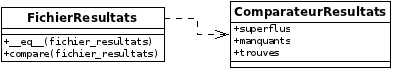
\includegraphics{figures/diagramme-classe-resultats.png}}
    \caption{Diagramme de classes du module résultats}
    \label{classesresultat}
\end{figure}


%\indent Les différentes architectures qui placent les services réseau au centre des décisions ont été rejetées car elles ne sont pas adaptées au présent problème. Deux styles d'architectures ont été évalués plus en détail: l'architecture en couches et l'architecture de type \emph{Pipes and Filters}.

%Dans une architecture en couches, chaque couche supplémentaire correspond à un degré d'abstraction plus élevé. Chacune des couches a une cohérence interne qui correspond à son degré d'abstraction du problème et est isolée des autres couches. L'interface de communication entre les différentes couches en est une de consommation de services, où chacune des couches fournit des services à sa couche supérieure. De bons exemples d'implémentation de cette architecture sont les modèles OSI et TCP/IP.

%Un exemple d'architecture en couche qui pourrait résoudre le problème est présenté dans la figure \ref{f1}. L'utilisateur utiliserait une interface graphique pour lancer une commande permettant de créer un document PDF à partir d'une image. Cette commande ferait appel à la couche «Construction de PDF» sachant que celle-ci fournit le service. Puisque la conversion d'une image en PDF passe par l'étape intermédiaire d'une conversion en LaTeX, la couche «Construction du document LaTeX» serait appellée pour fournir le service. Cette couche coordonnerait alors les appels vers les différents services de la couche inférieure, à savoir la reconnaissance de caractères, l'extraction de méta-données et l'acquisition des ressources bibliographiques. Enfin, ce serait le service de reconnaissance de caractères qui utiliserait la couche pré-traitement afin de faire les traitements nécessaires pour augmenter la précision de la reconnaissance de caractères (augmentation du contraste, alignement des colonnes, etc.). La couche « Numérisation » est déconnectée puisqu'elle est en quelque sorte optionnelle dans ce modèle, mais on pourrait concevoir que l'utilisateur puisse vouloir accéder à une fonction de type « Numériser un document».

%L'architecture \emph{Pipes and Filters} correspond à la métaphore d'un pipeline dans lequel l'information circulerait: le chemin est fixé et lorsque l'information a circulé, il n'y a pas de retour en arrière possible. Dans ce modèle, les filtres sont les logiciels qui modifient l'information et le pipeline est le canal de communication entre eux. La terminologie est en ce sens la même que celle des systèmes UNIX où ce type d'architecture est utilisé pour les commandes système. À titre d'exemple, on peut mentionner \emph{sed} et \emph{awk}.

%Dans notre cas, l'application de l'architecture \emph{Pipes and Filters} impliquerait que le problème soit décomposé en un ensemble de filtres ayant chacun une cohésion assez grande pour pouvoir être utilisé individuellement. Un exemple est proposé dans la Figure \ref{f2}. Deux processus ont été identifiés: le premier concerne l'extraction des méta-données et le deuxième concerne l'insertion des liens vers les ressources dans le document. Ils ont été séparés car l'insertion des hyperliens dans les documents est facultative et qu'il est difficile d'estimer le temps pour faire la recherche.

%Chacune de ces architecture a ses avantages. Dans une architecture en couches la solution est considérée comme un tout, tandis qu'avec une architecture de type \emph{Pipes and Filters} l'emphase est mise sur les propriétés des différents filtres. Nous estimons qu'il est plus facile de tenir compte des attributs qualité reliés à l'ergonomie et l'expérience utilisateur en ayant une vision holiste de la solution. En revanche, ce problème se prête bien à une architecture de type \emph{Pipes and Filters} puisque les filtres obtenus ont, à l'exception du filtre « Recherche de la ressource » car il dépend de ressources externes, les propriétés suivantes:

%\begin{itemize}
%    \item Sortie conditionnée uniquement par les entrées.
%    \item Aucun état à gérer
%    \item Aucune intervention de l'utilisateur (non-interactif) 
%\end{itemize}
%
%[expliquer pourquoi on conserve P\&F]
%
%Il est à noter cependant que notre modèle ne respecterait pas l'architecture \emph{Pipes and Filters} classique où l'information prend la forme d'un flux qui est \emph{immédiatement} envoyé au filtre suivant. Dans le cas qui nous intéresse, cela impliquerait que les caractères soient envoyés au filtre d'extraction de citations au fur et à mesure qu'ils sont reconnus. Or, il est plutôt nécessaire de considérer la page entière -- voir le chapitre, dans le cas où les citations seraient à la fin -- dans son ensemble pour pouvoir extraire les citations: l'information ne se trouve pas dans chaque caractère, mais plutôt dans la relation entre ceux-ci. Cette entorse au modèle ne devrait cependant pas poser problème dans la mesure où les critères énoncés ci-haut sont respectés.

%   \begin{figure}
%   \centerline{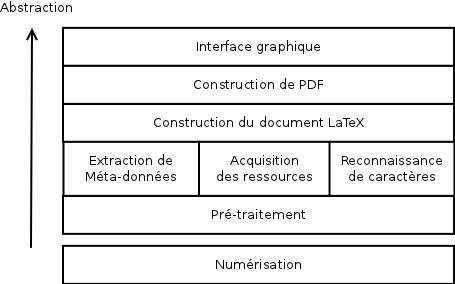
\includegraphics{figures/diagramme-couche.png}}
%    \caption{Exemple d'architecture en couche possible pour résoudre le problème}
%    \label{f1}
%    \end{figure}
%
%   \begin{figure}
%    \centerline{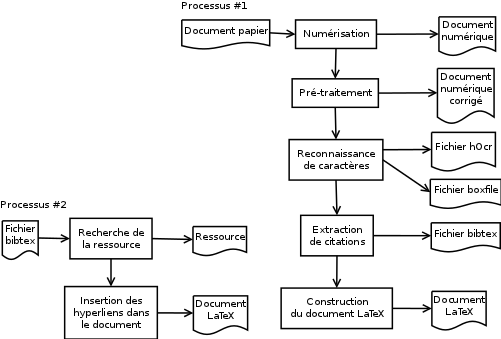
\includegraphics{figures/diagramme-flux.png}}
%    \caption{Exemple d'architecture de type \emph{Pipes and Filters} possible}
%    \label{f2}
%    \end{figure}


